\documentclass{beamer}
\usetheme{Madrid}
\usecolortheme{beaver}
\usepackage{amsthm,amsmath}
\usepackage{comment}
\usepackage{tikz}
\usetikzlibrary{calc,arrows.meta,positioning,shapes}
\usepackage{graphicx}
\usepackage[utf8]{inputenc}

\newtheorem{thm}{Theorem}
%\newtheorem{lemma}{Lemma}
\newtheorem{proposition}{Proposition}
\newtheorem{defn}{Definition}

\newcommand{\rs}[1]{{\color{red} RS:  #1}}

\newcommand{\cN}{\mathcal{N}}
\newcommand{\cO}{\mathcal{O}}
\newcommand{\bi}{\begin{itemize}}
	\newcommand{\ei}{\end{itemize}}


\title[Reinforcement Learning]{String Theory meets Machine Learning\\
	- Exploring Standard Like Models}
\author{Robin Schneider}
\institute{Uppsala University}
\date{November 2020}

\begin{document}
	
\frame{\titlepage}

\begin{frame}
\frametitle{Reinforcement learning}
What is reinforcement learning? \\
\bi
\item Optimal control of (in)completely-known Markov decision processes.
\item Training a learning agent to maximize a predefined goal by optimizing actions that manipulate its environment.
\item Third branch of machine learning.
\item Resembles most closely human learning.
\ei
\pause
Main challenge of reinforcement learning:
\bi
\item Balancing exploration and exploitation. A trade-off which has been studied for many years but remains unsolved.
\ei
\end{frame}

\begin{frame}
\frametitle{Why Reinforcement learning?}
Reinforcement Learning has a proven track record of beating us:
\bi
\item AlphaGo Zero - Won against world champion in GO, a game with $10^{170}$ valid board positions.
\item OpenAI Five - Won against world champions in DotA 2 {\color{blue}[1912.06680]}.
\ei
\pause 
Computations are plenty full:
\bi \item Up to $10^{428}$ topological inequivalent CY 3-folds {\color{blue} [2008.01730]} %https://inspirehep.net/literature/1810205
\item F-theory: $10^{272.000}$ flux vacua {\color{blue} [1511.03209]}%https://arxiv.org/abs/1511.03209
\ei 
\pause
Relevant applications for us:
\bi
\item Branes with Brains {\color{blue} [1903.11616]}
\item Explore and Exploit with Heterotic Line Bundle Models {\color{blue} [2003.04817]}
\item (Learning to Unknot {\color{blue} [2010.16263]})
\ei
\end{frame}


\begin{frame}
\frametitle{Markov Decision Process}
\begin{defn}
	A Markov decision process is a 4-tuple $(S, A, P_a, R_a)$, where
	\begin{itemize}
		\item $S$ is a set of states called the state space,
		\item $A$ is a set of actions called the action space,
		\item $P_a(s,s') = Pr(S_{t+1} = s'| S_t = s, A_t = a)$ is the probability of transitioning into state $s'$ given $s$ and $a$,
		\item $R_a(s,s')$ is the immediate reward for state transition $s \rightarrow s'$ due to action $a$.
	\end{itemize}
\end{defn}
%\textbf{Goal:} We want to maximize accumulated reward $G = \sum_t R_t$.
\end{frame}

\begin{comment}
\begin{frame}
\frametitle{An example MDP}
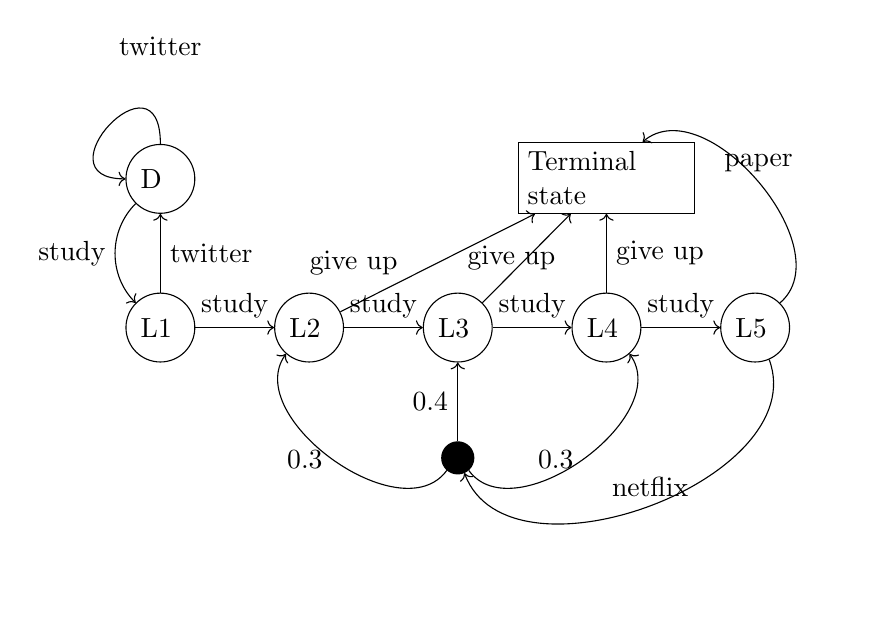
\begin{tikzpicture}
\node[draw,circle,text width=0.5cm] (1)
{L1 };
\node[draw,circle,text width=0.5cm] (2) [right =of 1]
{L2 };
\node[draw,circle,text width=0.5cm] (3) [right =of 2]
{L3 };
\node[draw,circle,text width=0.5cm] (4) [right =of 3]
{L4 };
\node[draw,circle,text width=0.5cm] (5) [right =of 4]
{L5 };
\node[draw,circle,text width=0.5cm] (6) [above =of 1]
{D };
\node[above = 1cm of 6] (6a){twitter};
\node[left = 1cm of 6] (6b){};
\node[draw,text width=2cm] (7) [above =of 4]
{Terminal state};
\node[draw,fill=black,circle,text width=0.1cm] (8) [below =of 3]
{ };	
\draw[->] (1) -- node[above] {study} (2);
\draw[->] (1) -- node[right, text width=1.5cm] {twitter} (6);
\draw[->] (6) to [bend left=315] node[left] {study} (1);
\draw[->] (6.north) ..  controls (6a) and (6b)  .. (6.west);
\draw[->] (2) -- node[above] {study} (3);
\draw[->] (3) -- node[above] {study} (4);
\draw[->] (4) -- node[above] {study} (5);
%\draw[->] (5) to [out=0,in=90] (7);
\draw[->] (5) to [bend left=270] node[above] {paper}(7);
\draw[->] (5) to [bend left=90] node[above] {netflix}(8);
\draw[->] (8) to [bend left=90] node[left] {0.3} (2);
\draw[->] (8) to node[left] {0.4} (3);
\draw[->] (8) to [bend right=90] node[left] {0.3} (4);
\draw[->] (3) to node[text width=1.5cm] {give up}(7);
\draw[->] (2) to node[left,text width=1.5cm] {give up}(7);
\draw[->] (4) to node[right, text width=1.5cm] {give up}(7);
\end{tikzpicture}
\end{frame}
\end{comment}

\begin{frame}
\frametitle{A familiar MDP}
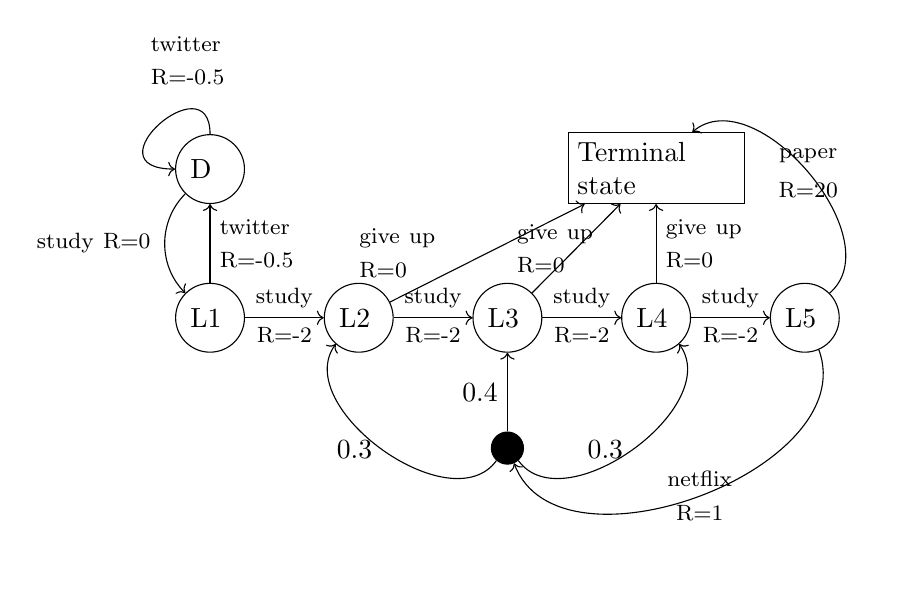
\begin{tikzpicture}
\node[draw,circle,text width=0.5cm] (1)
{L1 };
\node[draw,circle,text width=0.5cm] (2) [right =of 1]
{L2 };
\node[draw,circle,text width=0.5cm] (3) [right =of 2]
{L3 };
\node[draw,circle,text width=0.5cm] (4) [right =of 3]
{L4 };
\node[draw,circle,text width=0.5cm] (5) [right =of 4]
{L5 };
\node[draw,circle,text width=0.5cm] (6) [above =of 1]
{D };
\node[above = 0.5cm of 6, text width=1.5cm] (6a){\footnotesize twitter R=-0.5};
\node[left = 1cm of 6] (6b){};
\node[draw,text width=2cm] (7) [above =of 4]
{Terminal state};
\node[draw,fill=black,circle,text width=0.1cm] (8) [below =of 3]
{ };
\draw[->] (1) -- node[above] {\footnotesize study} node[below] {\footnotesize R=-2} (2);
\draw[->] (1) -- node[right, text width=1.5cm] {\footnotesize twitter R=-0.5} (6);
\draw[->] (6) to [bend left=315] node[left, text width=1.5cm] {\footnotesize study R=0} (1);
\draw[->] (6.north) ..  controls (6a) and (6b)  .. (6.west);
\draw[->] (2) -- node[above] {\footnotesize study} node[below] {\footnotesize R=-2} (3);
\draw[->] (3) -- node[above] {\footnotesize study} node[below] {\footnotesize R=-2} (4);
\draw[->] (4) -- node[above] {\footnotesize study} node[below] {\footnotesize R=-2} (5);
%\draw[->] (5) to [out=0,in=90] (7);
\draw[->] (5) to [bend left=270] node[above] {\footnotesize paper} node[below] {\footnotesize R=20}(7);
\draw[->] (5) to [bend left=90] node[above] {\footnotesize netflix} node[below] {\footnotesize R=1}(8);
\draw[->] (8) to [bend left=90] node[left] {0.3} (2);
\draw[->] (8) to node[left] {0.4} (3);
\draw[->] (8) to [bend right=90] node[left] {0.3} (4);
\draw[->] (3) to node[text width=1.5cm] {\footnotesize give up R=0}(7);
\draw[->] (2) to node[left,text width=1.5cm] {\footnotesize give up R=0}(7);
\draw[->] (4) to node[right, text width=1.5cm] {\footnotesize give up R=0}(7);
\end{tikzpicture}
\end{frame}

\begin{frame}
\frametitle{Policy}
How to pick actions?
\begin{defn}
	A policy $\pi$ is a distribution over actions given states,
	\begin{align}
	\pi (a|s) = \mathbb{P}[A_t = a| S_t = s]
	\end{align}
\end{defn}
\pause
%Want to maximize:
\begin{defn}
The return $G_{t}$ is the total discounted reward for time-step $t$.
\begin{align}
G_{t} = R_{t+1} + \gamma  R_{t+2} + ... = \sum_{k} \gamma^{k} R_{t+k+1} , \qquad \text{ with } \gamma \in [0,1]
\end{align}
\end{defn}
\end{frame}

\begin{frame}
\frametitle{State value function}
\begin{defn}
	The state value function $v_\pi(s)$ of an MDP is the expected return starting from state $s$ and following policy $\pi$
	\begin{align}
		v_\pi(s) = \mathbb{E}_\pi[G_t | S_t = s]
	\end{align}
\end{defn}
\pause
\begin{defn}
	The action value function $q_\pi(s, a)$ of an MDP is the expected return starting from state $s$, using action $a$, and then following policy $\pi$
	\begin{align}
	q_\pi(s,a) = \mathbb{E}_\pi[G_t | S_t = s, A_t = a]
	\end{align}
\end{defn}
\end{frame}

\begin{frame}
\frametitle{Bellman equation}
How to compute state value function?

Use \textbf{Bellman equations}:
\begin{align}
v_\pi(s) & = \mathbb{E}_\pi[G_t | S_t = s] = \mathbb{E}_\pi[R_{t+1} + \gamma R_{t+2} + ... | S_t = s] \nonumber \\
& = \mathbb{E}_\pi[R_{t+1} + \gamma v(s_{t+1}) + ... | S_t = s] 
\end{align}
and 
\begin{align}
q_\pi(s,a) & = \mathbb{E}_\pi[R_{t+1} + \gamma q_\pi (S_{t+1}, A_{t+1}) | S_t = s, A_t = a] 
\end{align}
\pause
Example \textbf{STmML}. Take a uniform policy and $\gamma = 1$:
\begin{align}
	v(L_5) = \frac{1}{2} \cdot 20 + \frac{1}{2} \left[1 + \frac{3}{10} v(L_2) + \frac{4}{10} v(L_3) + \frac{3}{10} v(L_4) \right]
\end{align}
\end{frame}

\begin{frame}
\frametitle{MDP with $v(s)$}
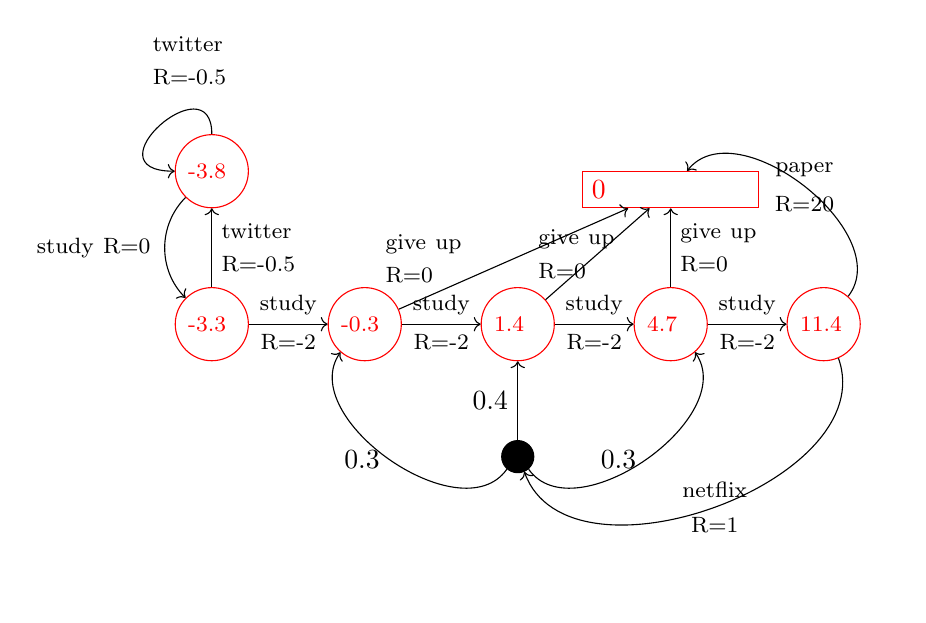
\begin{tikzpicture}
\node[draw,circle,text width=0.6cm,color=red] (1)
{\footnotesize -3.3};
\node[draw,circle,text width=0.6cm,color=red] (2) [right =of 1]
{\footnotesize -0.3};
\node[draw,circle,text width=0.6cm,color=red] (3) [right =of 2]
{\footnotesize 1.4};
\node[draw,circle,text width=0.6cm,color=red] (4) [right =of 3]
{\footnotesize 4.7};
\node[draw,circle,text width=0.6cm,color=red] (5) [right =of 4]
{\footnotesize 11.4};
\node[draw,circle,text width=0.6cm,color=red] (6) [above =of 1]
{\footnotesize -3.8};
\node[above = 0.5cm of 6, text width=1.5cm] (6a){\footnotesize twitter R=-0.5};
\node[left = 1cm of 6] (6b){};
\node[draw,text width=2cm,color=red] (7) [above =of 4]
{0};
\node[draw,fill=black,circle,text width=0.1cm] (8) [below =of 3]
{ };
\draw[->] (1) -- node[above] {\footnotesize study} node[below] {\footnotesize R=-2} (2);
\draw[->] (1) -- node[right, text width=1.5cm] {\footnotesize twitter R=-0.5} (6);
\draw[->] (6) to [bend left=315] node[left, text width=1.5cm] {\footnotesize study R=0} (1);
\draw[->] (6.north) ..  controls (6a) and (6b)  .. (6.west);
\draw[->] (2) -- node[above] {\footnotesize study} node[below] {\footnotesize R=-2} (3);
\draw[->] (3) -- node[above] {\footnotesize study} node[below] {\footnotesize R=-2} (4);
\draw[->] (4) -- node[above] {\footnotesize study} node[below] {\footnotesize R=-2} (5);
%\draw[->] (5) to [out=0,in=90] (7);
\draw[->] (5) to [bend left=270] node[above] {\footnotesize paper} node[below] {\footnotesize R=20}(7);
\draw[->] (5) to [bend left=90] node[above] {\footnotesize netflix} node[below] {\footnotesize R=1}(8);
\draw[->] (8) to [bend left=90] node[left] {0.3} (2);
\draw[->] (8) to node[left] {0.4} (3);
\draw[->] (8) to [bend right=90] node[left] {0.3} (4);
\draw[->] (3) to node[text width=1.5cm] {\footnotesize give up R=0}(7);
\draw[->] (2) to node[left,text width=1.5cm] {\footnotesize give up R=0}(7);
\draw[->] (4) to node[right, text width=1.5cm] {\footnotesize give up R=0}(7);
\end{tikzpicture}
\end{frame}

\begin{frame}
\frametitle{Optimal value function and policy}
\begin{defn}
	The optimal state value function $v_*(s)$ is the maximum value function over all policies
	\begin{align}
	v_*(s) = \underset{\pi}{\max} \; v_\pi(s).
	\end{align}
\end{defn}
\begin{thm}
	Define a partial ordering over policies
	\begin{align}
		\pi \geq \pi' \text{ if } v_\pi (s) \geq v_{\pi'}(s) \; \forall \; s.
	\end{align}
	Then for any Markov decision process
	\bi
	\item exists an optimal policy $\pi_*$ that is better than or equal to all other policies, $\pi_* \geq \pi \; \forall \; \pi$,
	\item all optimal policies achieve the optimal value function $v_{\pi_*} (s) = v_* (s)$.
	\ei
\end{thm}
\end{frame}

\begin{frame}
\frametitle{Literature}
How do we find the optimal policy or state value function? By consulting the literature :)
\begin{itemize}
	\item Youtube Lecture series: David Silver - Introduction to Reinforcement Learning
	\item Book: Sutton and Barto - Introduction to Reinforcement Learning
	\item (Optional) Interdisciplinary course at Uppsala University 
\end{itemize}
\end{frame}

\begin{frame}
\frametitle{Actor Critic models}
What happens if our state space is too vast to store in memory or too large to explore at all? Neural networks come to our rescue, we can approximate $\pi$ or $v_\pi(s)$ (deep reinforcement learning).
\pause

Asynchronous Advantage Actor Critic (A3C) surpassed state of the art performance in many benchmarks {\color{blue}[1602.01783]}. They
\begin{itemize}
	\item use a NN as Actor to update $\pi$,
	\item use a NN as Critic to update $q_\pi(s,a)$,
	\item can be trained on a single CPU by updating global parameters asynchronously from local agents,
	\item are stable and robust (on considered benchmarks).
\end{itemize}
\end{frame}


\begin{frame}
\frametitle{A game}
\begin{figure}
	\centering
	\includegraphics[scale=0.3]{pregame.png}
	\caption{\it Who finds the most realistic string vacua?}
\end{figure}
\end{frame}


\begin{frame}
\frametitle{Standard like models}
Heterotic string compactification with three ingredients {\color{blue} [1106.4804,1202.1757,1307.4787]}.
\begin{enumerate}
	\item Calabi Yau manifold $M$. \item Line bundle sum $V = \otimes_{a=1}^5 L_a$. \item Freely acting discrete symmetry $\Gamma$ for Wilson line.
\end{enumerate}
For example:
\begin{align}
\mathcal{M}_{5302} =  \left[
\begin{array}{c||ccc}
1 & 0 & 1 & 1 \\
1 & 0 & 1 & 1 \\
1 & 1 & 1 & 0 \\
1 & 1 & 1 & 0 \\
1 & 1 & 0 & 1 \\
1 & 1 & 0 & 1
\end{array}
\right]^{6,30}_{-48} \text{ and }  V = \left[\begin{array}{ccccc}
-1& 0& 0& 0& 1\\ 
4& -3& -1& 0& 0\\ 
0& 0& -1& 1& 0\\ 
0& 0& 0& 0& 0\\ 
0& 0& 1& 0& -1\\ 
1& 1& 0& -2& 0
\end{array}\right]\nonumber 
\end{align}
and $|\Gamma| = 2$. There are a total of 6294 such models.
\end{frame}

\begin{frame}
\frametitle{Reward structure}
	\begin{enumerate}
	\item $V$ has to be an $S(U(1)^5)$ bundle, thus $c_1(V) = 0$. R$_{\text{max}}$=5. \label{c:sun}
	\item The \textit{weak} stability constraint; each line bundle has slope zero somewhere in the K\"ahler cone; $\mu(L_a)=0, a=1,...,5$. R$_{\text{max}}$=2. \label{c:weak}
	\item There are three fermionic matter generations; the index of each line bundle is in the range $-3 |\Gamma| \leq \text{index}(L_a) \leq 0$, where $|\Gamma|$ is the rank of the freely acting symmetry.  R$_{\text{max}}$= $10$. \label{c:index}
	\item There are three fermionic matter generations; the index of $V$ is determined by $\text{ind} (V) \stackrel{!}{=} -3 |\Gamma|$. R=$10^2$. \label{c:Index}
	\item The Bianchi identity and Bogomolov bounds impose $0 < c_2(V) \leq c_2 (\mathcal{M})$. R=$10^4$. \label{c:bianchi}
	\item Exclude exotic Higgs triplets; $\text{ind}(L_a \otimes L_b) < 0$. R=$10^4$.\label{c:triplet}
	\item Require at least one Higgs doublet; $h^2(\wedge^2 V) \geq 0$. 
	R=$10^6$.\label{c:doublet}
	\item There are no antigenerations, $h^2(V) \stackrel{!}{=} 0$. R=$10^7$.\label{c:fermion}
	%\item $V$ needs to admit an equivariant structure.
	\item $V$ needs to be slope stable somewhere in the K\"ahler cone. \label{c:kaehler}
\end{enumerate}
\end{frame}



\begin{frame}
\frametitle{Stacking I}
\textbf{Environment:} Stacking of line bundles $L_{1-4}$ on top of each other.

\textbf{Observation space:} The line bundle sum $V$. Hence $S_t \sim \mathbb{Z}^{(5 , \text{nProj})}$. 

\textbf{Action space:} Pick a slope stable line bundle with $h^1(L) \leq 3 |\Gamma|$ from a precompiled list of $n_{\text{line}}$ line bundles.

\textbf{\# of configurations:} $n_{\text{conf}} = n_{\text{line}}^4$. Take e.g. 5302 with max charge $q_{\text{max}} = 2$ and $|\Gamma| = 2$, then $n_{\text{line}} = 2890$ and $n_{\text{conf}} \approx 7 \cdot 10^{13}$.\\

\textbf{Example}:
\begin{align}
\small
 \left[\begin{array}{ccccc}
-1& 0& 0& 0& 1\\ 
2& 0& -1& -1& 0\\ 
-2& -1& 0& -2& 5\\ 
0& -1& 0& 2& -1\\ 
0& 2& -2& 2& -2\\ 
2& 2& 1& 0& -5
	\end{array}\right] \stackrel{A_t = 7}{\rightarrow} \left[\begin{array}{ccccc}
-1& -2& 0& 0& 3\\ 
2& -2& -1& -1& 2\\ 
-2& 0& 0& -2& 4\\ 
0& 2& 0& 2& -4\\ 
0& 0& -2& 2& 0\\ 
2& 2& 1& 0& -5
	\end{array}\right]
\end{align}
\end{frame}

\begin{frame}
\frametitle{Stacking II}
\begin{figure}[t]
	
	\centering
	\begin{minipage}{0.47\linewidth}
		\includegraphics[scale=0.4]{5256_s4p1r_30_5_range.pdf}
	\end{minipage}
	\begin{minipage}{0.47\linewidth}
		\includegraphics[scale=0.4]{5302_s4p1r_30_5_range.pdf}
	\end{minipage}
	
	\caption{\it Number of models found in two selected sets of stacking experiments (in blue) for the manifolds 5256 and 5302 plotted for comparison with each five random walkers (in red).}
	\label{fig: stack}
\end{figure}
\end{frame}

\begin{frame}
\frametitle{Half time}
\begin{figure}
	\centering
	\includegraphics[scale=0.3]{midgame.png}
	\caption{\it An early lead.}
\end{figure}
\end{frame}

\begin{frame}
\frametitle{Flipping I}
\textbf{Environment:} Flipping of charges $q_i^j$ in $L_{1-4}$.

\textbf{Observation space:} The line bundle sum $V$. Hence $S_t \sim \mathbb{Z}^{(5 , \text{nProj})}$.

\textbf{Action space:} Pick a charge $q_i^j$ and add $\pm 1$. Thus there are $A_t \in \{1, ..., 4 \cdot 2 \cdot \text{nProj} \}$ actions.

\textbf{\# of configurations:} $n_{\text{conf}} = (2 \cdot q_{\text{max}} +1)^{4 \cdot h^{1,1}}$. Take e.g. 5302 with max charge $q_{\text{max}} = 2$, then $n_{\text{conf}} \approx 5 \cdot 10^{16}$.

\textbf{Example}:
\begin{align}
\small
\left[\begin{array}{ccccc}
1& 1& -1& 0& -1\\ 
-1& 0& 1& 0& 0\\ 
1& 1& 0& -1& -1\\ 
1& 1& -1& -1& 0\\ 
-1& 1& 0& 0& 0\\ 
-1& 1& 0& 0& 0
\end{array}\right] \stackrel{A_t = 0}{\rightarrow} \left[\begin{array}{ccccc}
2& 1& -1& 0& -2\\ 
-1& 0& 1& 0& 0\\ 
1& 1& 0& -1& -1\\ 
1& 1& -1& -1& 0\\ 
-1& 1& 0& 0& 0\\ 
-1& 1& 0& 0& 0
\end{array}\right]
\end{align}
\end{frame}

\begin{frame}
\frametitle{Flipping II}
\begin{figure}[ht]
	
	\centering
	\begin{minipage}{0.47\linewidth}
		\includegraphics[scale=0.4]{5256_f4p1_200_5_range.pdf}
	\end{minipage}
	\begin{minipage}{0.47\linewidth}
		\includegraphics[scale=0.4]{5302_f4p1_300_5_range.pdf}
	\end{minipage}
	
	\caption{\it Number of models found in two selected sets of flipping experiments (in blue) for the manifolds 5256 and 5302 plotted for comparison with each five random walkers (in red).}
	\label{fig: flip}
\end{figure}
\end{frame}

\begin{frame}
\frametitle{Transfer learning}
\begin{figure}[t]
	
	\centering
	\begin{minipage}{0.47\linewidth}
		\includegraphics[scale=0.4]{5452_f4p1_200_5_range_log.pdf}
	\end{minipage}
	\begin{minipage}{0.47\linewidth}
		\includegraphics[scale=0.4]{6890_f4p1_200_5_range_log.pdf}
	\end{minipage}
	
	\caption{\it Number of models found for selected sets of flipping experiments (in blue), random walkers (in red), pretrained agents (in yellow), and transfer agents (in green) on the manifolds 5452 and 6890. Note the logarithmic scale on the y-axis.}
	\label{fig: transfer}
\end{figure}
\end{frame}

\begin{frame}
\frametitle{Final Score}
\begin{figure}
	\centering
	\includegraphics[scale=0.3]{endgame.png}
	\caption{\it Looks like a draw to me.}
\end{figure}
\end{frame}


\end{document}